\chapter{Effective Multiclass Transfer For Hypothesis Transfer Learning}\label{sec:pakdd}
\section{Introduction}
Domain adaptation for image recognition tries to exploit the knowledge from a source domain with plentiful data to help learn a classifier for the target domain with a different distribution and little labeled training data. In domain adaptation, the source and target domains share the same label but their data are drawn from different distributions.

Previous research \cite{ben2010theory,ben2007analysis} shows that without carefully measuring the distribution similarity between the source and target data, the source knowledge could not be exploited effectively or even hurt the learning process (called  \textit{negative transfer})\cite{pan2010survey}. 
However, as we are not able to access the source data in the Hypothesis Transfer Learning (HTL) \cite{kuzborskij2013stability} setting, how to effectively and safely exploit the knowledge from the source model could be an important issue in HTL, especially when target data is relatively small (Effectiveness issue). Moreover, the source models from different domains can be trained with different kinds of classifiers. For example most models trained from ImageNet are deep convolutional neural networks while some models of the VOC recognition task could be SVMs or ensemble models. Therefore, a practical HTL algorithm should be compatible with different types of source classifiers (Compatibility issue). Previous work is limited to either leveraging the knowledge from certain type of source classifiers \cite{tommasi2014learning,fei2006one} or low transfer efficiency in a small training set\cite{jie2011multiclass}. To the best of our knowledge, none of the previous work in HTL is able to solve these two issues at the same time.

In this chapter, we propose our method, called \textbf{Effective Multiclass Transfer Learning} (EMTLe), that can solve these two issues simultaneously. We perform comprehensive experiments on 4 real-world datasets from two benchmark datasets (3 from Office and 1 from Caltech256). We show that EMTLe can effectively transfer the knowledge with different types of source models and outperforms the baseline methods under the HTL setting.

\section{Using the Source Knowledge as the Auxiliary Bias}\label{sec:prob}
%In this section, we introduce our strategy in EMTLe that can exploit the knowledge from different types of source classifiers. In general, for each example in the target domain, we use its output class probabilities from the source models as the auxiliary bias term to adjust the final prediction of the target model.

\begin{figure}
	\centering
	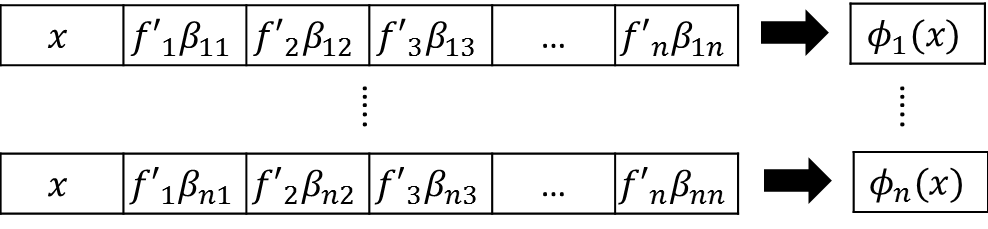
\includegraphics[scale=0.4]{pakdd/fig/mktl.png}
	\caption{Illustration of feature augmentation in MKTL. $f_i'$ is the output of the $i$-th source model and $\beta_{in}$ is the hyperparameter (need to be estimated) to weigh the augmented feature. $\phi_n(x)$ is augmented feature for the $n$-th binary model.}
	\label{fig:mktl}
\end{figure}
Some previous work such as MKTL\cite{jie2011multiclass} suggests that using the prediction from the source model as the source knowledge can greatly release the constraint of the type of the source model. However, with complex feature augmentation method, there are many hyperparameters to be estimated which makes it inefficient with small training set. In this paper, we adopt the idea of using the source model prediction as the transferable knowledge and propose our transfer strategy.

Suppose we have to recognize a image from one of the $N$ visual classes and there are $N$ experts each of who can only provide the probability of this image for one certain class (binary source model). After we make our decision for one example (prediction from target model), the experts provide their own decisions as well (probabilities from the source models). Their decisions can provide extra information regarding this example as the auxiliary bias and adjust our final prediction.
As each of the experts is a specialist in one class, we should weigh their decisions as well due to the bias of their predictions (see Figure \ref{fig:ab}). 

Unlike previous work\cite{aytar2011tabula,tommasi2014learning,yang2007adapting} which has to use the specific parameter of the source model as the source knowledge, our strategy is more compatible with different types of classifiers. Compared to MKTL\cite{jie2011multiclass}, we only have to estimate $N$ hyperparameters for the $N$-class problem while there are \mbox{$N\times N$} hyperparameters in MKTL (see Figure \ref{fig:mktl}). Therefore, it is easier to estimate the transfer parameters with our strategy and EMTLe can perform better especially when the size of the training set is small.
In addition, there are two advantages of our strategy: (1) It is an effective and easy way to align the knowledge from different types of source classifiers.
(2) The auxiliary bias term is naturally normalized in the same dimension as the class probabilities are always in the interval $[0,1]$.  As EMTLe can select more types of source classifiers, this makes it more practical in a real HTL scenario.

\begin{figure}
	\centering
	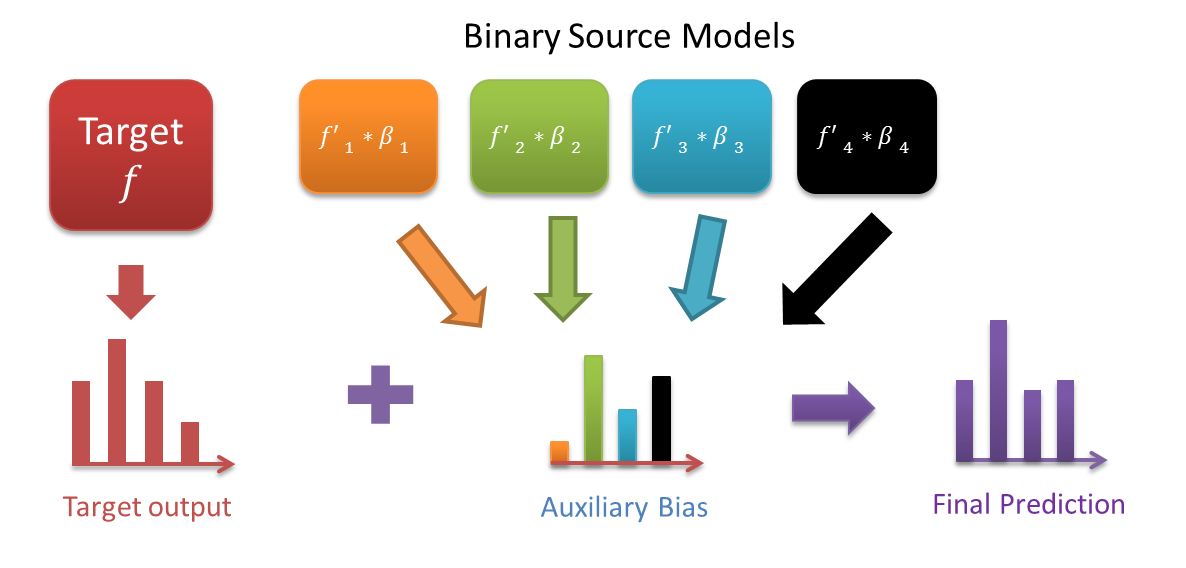
\includegraphics[scale=.7]{pakdd/fig/ab.png}
	\caption{Demonstration of using the source class probability as the auxiliary bias to adjust the output of the target model.}% $f'$ is a group of binary classifiers $\{f'_1,...,f'_4\}$ for each class and for each source model $f'_n$, we use the weight $\beta_n$ to control the knowledge transferred from this model.}
	\label{fig:ab}
\end{figure}


Here, the weight of each source model reflects the relatedness between the source model and our target domain. The more related they are, the better decision the source model can make and the larger weight we should apply to it. Specifically, in this paper, we call the weight \textit{transfer parameter}. Therefore, for any target data $D=\{x,y\}$ and the given source models $f'=\{f'_1,...,f'_N\}$, our goal is to find the target model $f$:
\begin{equation}\label{eq:low_opt}
f=\underset{f \in \mathcal{F}}{\arg \min}\ell\left(f+\beta f'|D,\beta\right)
\end{equation} 
where $\beta=[\beta_1,...,\beta_N]$ is the transfer parameter and $\ell(\cdot,\cdot)$ is the loss function to learn the target model.
It is obvious that assigning the proper transfer parameter to the source model can significantly improve the performance of our final prediction.
From Eq. \eqref{eq:low_opt} we can see that, once we have determined the value of the transfer parameter $\beta$, we are able to find the target model $f$ and solve the learning problem.
However, the transfer parameter in Eq.\eqref{eq:low_opt} is a hyperparameter and we cannot solve it directly. Therefore, we introduce our bi-level optimization method for transfer parameter estimation in the next section.









\section{Bi-level Optimization for Transfer Parameter Estimation}\label{sec:smitle}
As we discussed before, the transfer parameter in Eq. \eqref{eq:low_opt} is a hyperparameter that cannot be solved directly. 
Here we use bi-level optimization (\textbf{BO})\cite{Pedregosa16}, a popular method that is used in hyperparameter optimization to estimate the transfer parameter. In BO, the low-level optimization problem is to learn the target model and the high-level problem is another cross-validation (CV) hyperparameter optimization problem corresponding to the model learned at the low-level.

\begin{figure}[h]
	\centering
	\includegraphics[scale=.7]{pakdd/fig/bo.png}
	\caption{Bi-level Optimization problem for EMTLe.}% $f'$ is a group of binary classifiers $\{f'_1,...,f'_4\}$ for each class and for each source model $f'_n$, we use the weight $\beta_n$ to control the knowledge transferred from this model.}
	\label{fig:pakdd:bo}
\end{figure}

Suppose we use K-fold CV on the high-level problem. For the $i$-th fold CV, the target set $D$ is split into training set $D_i^{tr}$ and validation set $D_i^{val}$. The transfer parameter can be optimized with the following BO function:
\begin{equation}\label{eq:BO}
\begin{aligned}
\text{High level}\qquad&\beta=\underset{\beta}{\arg \min}\sum_i^K\mathcal{L}(f^{i}(\beta)|D_i^{val})\\
\text{Low level}\qquad&f^{i}(\beta)=\underset{f \in \mathcal{F}}{\arg \min}\ell\left(f+\beta f'|D_i^{tr},\beta\right) 
\end{aligned}
\end{equation} 
Here, $\ell(\cdot,\cdot)$ and $\mathcal{L}(\cdot,\cdot)$ are our low-level and high-level objective functions respectively. We can use any convex loss functions in Eq.\eqref{eq:BO} for optimization (e.g. SVM objective function). In this paper, we use the leave-one-out cross-validation (\textbf{LOOCV}) in the high-level problem. Previous research \cite{kuzborskij2013stability} suggests that LOOCV can increase the robustness of the estimated hyperparameter especially on the small dataset.
In previous studies\cite{maclaurin2015gradient,Pedregosa16}, BO is a non-convex problem and can only obtain the local optimal solution. However, we will show that problem \eqref{eq:BO} is strongly convex and we are able to obtain its optimal solution. 
\subsection{Low-level optimization problem}
To better illustrate our learning scenario, we define our learning process as follows. Suppose we have $N$ visual categories and 
can obtain $N$ source binary classifiers $f'=\{f'_1,...,f'_N\}$ from the source domain. We want to train a target function $f$ consisting of $N$ binary classifiers $f=\{f_1,...,f_N\}$ using the target training set $D$ and the source models $f'$.
Specifically, in our BO problem Eq. \eqref{eq:BO}, for the low-level optimization, we consider the scenario where we have to train $N$ binary linear target models $f_i = w_ix+b_i$ so that for any $\{x_i,y_i\}_{i=1}^l \in D$, the adjusted result satisfies $f(x)+f'(x)\beta = y$. Let $D^{\backslash i} = D\backslash\{x_i,y_i\}$.
Then, we use mean square loss in the low-level objective function to optimize each target model $f_n$ with any given transfer parameter $\beta$:
\begin{equation}\label{eq:bo_low}
\begin{aligned}
\text{Low-level:}\quad&f^{\backslash i}(\beta) : \underset{w,b}{\min} \sum_n^N\frac{1}{2}||w_n||^2+\frac{C}{2}\sum_je^2_{jn}\\
%\left(Y_{jn}-f_n(x_j)-\beta_n f_n'(x_j)\right)^2\\
\text{s.t.} &\qquad f_n(x) = w_nx+b_n; \quad x_j \in D^{\backslash i}\\
&\qquad e_{jn} = Y_{jn}-f_n(x_j)-\beta_n f_n'(x_j)
\end{aligned}
\end{equation}
Here, $Y$ is an encoded matrix of $y$ using the one-hot strategy where $Y_{in} =1$ if $y_i=n$ and 0 otherwise.

The reason why we use the objective function \eqref{eq:bo_low} is that it can provide an unbiased closed form Leave-one-out error estimation for each binary model $f_n$\cite{cawley2006leave}. As a result, the high-level problem becomes a convex problem and we are able to estimate our transfer parameter easier.

Let $K(X,X)$ be the kernel matrix and $C$ be the penalty parameter in Eq.\eqref{eq:bo_low}. We have:
\begin{equation}\label{eq:linear}
\psi=\left[ 
{K(X,X) + \frac{1}{C}{\rm{I}}} \right]
\end{equation}
Let $\psi^{-1}$ be the inverse of matrix $\psi$ and  $\psi_{ii}^{-1}$ is the $ith$ diagonal element of $\psi^{-1}$. $\hat{Y}_{in}$, the LOO estimation of binary model $f^{\backslash i}_n$ for sample $x_i$, can be written as\cite{cawley2006leave}:
\begin{equation} \label{eq:loo}
{\hat Y_{in}} = {Y_{in}} - \frac{{{\alpha _{in}}}}{{\psi_{ii}^{ - 1}}}\quad {\text{for}}\quad n = 1,...,N
\end{equation}
where the matrix $\boldsymbol{\alpha}=\{\alpha_{in}|i=1,...l;n=1,...,N\}$ can be calculated as:
\begin{equation}
\boldsymbol{\alpha} =\psi^{-1} Y - \psi^{-1} f'(X)diag(\boldsymbol{\beta})
\end{equation}

\subsection{High-level optimization problem} 
For the high level optimization problem, we use multi-class hinge loss \cite{crammer2002algorithmic} with $\ell_2$ penalty in our objective function.
\begin{equation}\label{eq:bo_high}
\begin{aligned}
\text{High-level:}\quad&\beta: \min \frac{{{\lambda}}}{2}\sum\limits_{n}^N {{{\left\| {{\beta _n}} \right\|}^2}}  +
\sum_i\xi_i\\
%\sum\limits_{i,n}\left[ {1 - {\varepsilon _{n{y_i}}} + {{\hat Y}_{in}} - {{\hat Y}_{i{y_i}}} - {\xi _i}} \right]\\
\text{s.t.} \qquad& 1 - {\varepsilon _{n{y_i}}} + {\hat Y_{in}} - {\hat Y_{i{y_i}}} \le {\xi_i}
\end{aligned}
\end{equation}
Here, $\varepsilon _{n{y_i}}=1$ if $n=y_i$ otherwise 0.
$\lambda$ is used to balance the $\ell_2$ penalty and our multi-class hinge loss. 
Compared to the previous work \cite{kuzborskij2013n,tommasi2014learning} which uses the multi-class hinge loss without the $\ell_2$ penalty, there are two main advantages for our high-level objective function: 
\begin{enumerate}
	\item When the training set is small, our LOOCV estimation could have a large variance. It is important to add the $\ell_2$ penalty to {reduce the variance and improve the generalization ability of the estimated transfer parameter}.
	\item It is clear that $\hat{Y}$ is a linear function w.r.t. $\beta$. With the $\ell_2$ penalty, the high-level optimization problem \eqref{eq:bo_high} becomes a strongly convex optimization problem w.r.t. the transfer parameter $\beta$.Therefore, we can obtain an $O({\log(t)}/{t})$ optimal solution with $t$ iterations using Algorithm \ref{alg:1} (see proof of Theorem \ref{th:1} in Appendix).
\end{enumerate}



\begin{algorithm}\label{alg:1}
       \caption{EMTLe}\label{alg:1}
        \begin{algorithmic}[1]
            \REQUIRE $\lambda, \psi,Y,f',T$,
            \ENSURE $\beta=\left\{\beta^1,...,\beta^n\right\}$
            \STATE $\beta^0 = 1$
            ,$\alpha' = \psi^{-1}Y,\alpha'' = \psi^{-1}f'$
            \FOR {$t=1$ to $T$}
                \STATE $\hat Y \leftarrow Y - {\left( {\psi^{-1} \circ I} \right)^{ - 1}}\left( \alpha' - \alpha''diag(\beta) \right)$
                %\STATE ${\Delta _\beta }=0$ 
                \FOR {$i=1$ to $l$}
                	\STATE ${\Delta _\beta }=\lambda\beta$ 
                	%\FOR {$r=1$ to $N$}
	                    \STATE $l_{ir} = \max(1 - {\varepsilon _{{y_i}r}} + {\hat Y_{ir}} - {\hat Y_{i{y_i}}})$
	                    \IF{$l_{ir}>0$}
	                            \STATE $\Delta _\beta^{{y_i}} \leftarrow \Delta _\beta^{{y_i}} - \frac{{{\alpha''_{i{y_i}}}}}{{{\psi^{-1}_{ii}}}}$%
	                            , $\Delta _\beta^{{r}} \leftarrow \Delta _\beta^{{r}} + \frac{{{\alpha''_{i{r}}}}}{{{\psi^{-1}_{ii}}}}$%
	                    \ENDIF
	                 %\ENDFOR %class ends   
                \ENDFOR %examples ends
                \STATE $\beta^t  \leftarrow \beta^{(t-1)}  - \frac{{{\Delta _\beta }}}{{\lambda\times {t} }}$
             \ENDFOR %iteration ends
        \end{algorithmic}
\end{algorithm} 
%\input{smitle.tex}

\section{Experiments}\label{sec:exp}
In this section, we show empirical results of our algorithm for different transferring situations on two image benchmark datasets: Office and Caltech.
\subsection{Dataset \& Baseline methods}
Office contains 31 classes from 3 subsets (Amazon, Dslr and Webcam) and Caltech contains 256 classes. We select 13 shared classes from two datasets\footnote{13 classes include: backpack, bike, helmet, bottle, calculator, headphone, keyboard, laptop, monitor, mouse, mug, phone and projector}. The input features of all examples are extracted using AlexNet\cite{krizhevsky2012imagenet}.
%Because the two subsets Dslr and Webcam are relatively small and don't have data for testing, we only use them as the source domain.
\begin{table}[htbp]
	\centering
	\caption{Statistics of the datasets and subsets}
	\begin{tabular}{|c|c|c|c|c|}
		\hline
		Dataset&Subsets&\# classes &\# examples & \# features\\\hline
		\multirow{3}{*}{Office} & Amazon (A) &13&1173 & 4096\\
		
		& Dslr (D) &13&224 & 4096\\
		& Webcam (W) &13&369 & 4096\\
		\hline
		Caltech256&Caltech (C)&13&1582&4096\\
		\hline
	\end{tabular}%
	\label{tab:class_info}%
\end{table}%
We compare our algorithm EMTLe with two kinds of baselines. The first one is the methods without leveraging any source knowledge (no transfer baselines), including two methods. \textbf{No transfer:} SVMs trained only on target data. Any transfer algorithm that performs worse than it suffers from negative transfer. \textbf{Batch:} We combine the source and target data, assuming that we have full access to all data, to train the SVMs. The result of the Batch method is expected to outperform other methods under the HTL setting as it can access the source data. The second kind of baseline consists of two previous transfer methods in HTL, \textbf{MKTL\cite{jie2011multiclass}} and \textbf{Multi-KT\cite{tommasi2014learning}}. Similar to EMTLe, both of them use the LOOCV method to estimate the relatedness of the source model and target domain, but they use their convex objective function without the $\ell_2$ penalty terms. We use linear kernel for all methods in all our experiments.
\subsection{Transfer from Single Source Domain}
In this subsection, following the experiment protocol in \cite{jie2011multiclass,tommasi2014learning} for a fair comparison, we perform 12 groups of experiments under the setting of HTL. 
For each experiment, one of the 4 (sub)datasets is selected as the source, while another dataset is used as the target. We evaluate the performance of EMTLe when all source models are of the same type. As Multi-KT can only leverage knowledge when the source model is SVM, All source models are trained with linear SVMs.
The size of each target dataset is varied from 1 to 5 to see how EMTLe and other baselines behave under the extremely small dataset. We use a heuristic way to set the value of $\lambda$ in Eq. \eqref{eq:bo_high}:
\begin{equation}
\lambda = 2e^{err_{n}-err_{s}}
\end{equation}
where $err_{n}$ and $err_{s}$ denote the performance of ``No transfer'' and the source model on the training set.
We perform each experiment 10 times and report the average result in Figure \ref{fig:exp}. 
\begin{figure}[th]
\centering
\subfloat[C$\rightarrow$A]{
    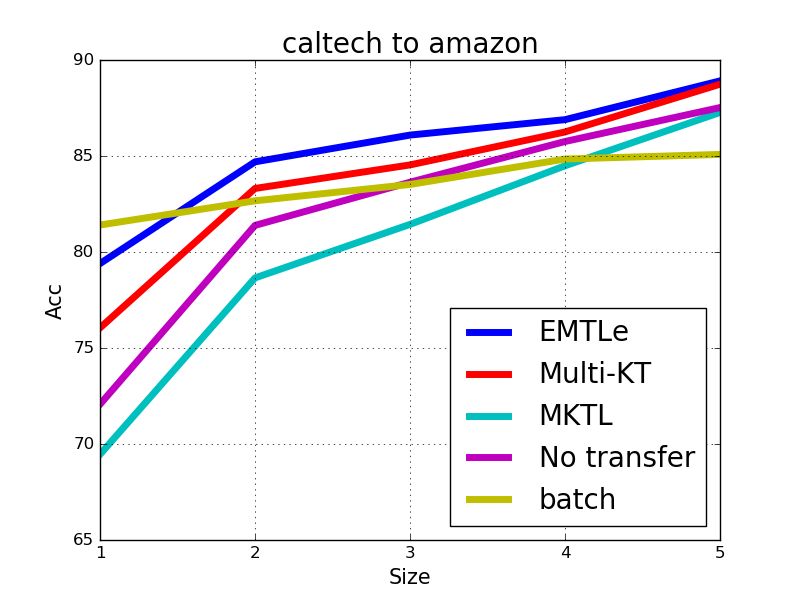
\includegraphics[width=0.30\textwidth]{pakdd/fig/caltechtoamazon.png}\label{a}
}
\subfloat[D$\rightarrow$A]{
    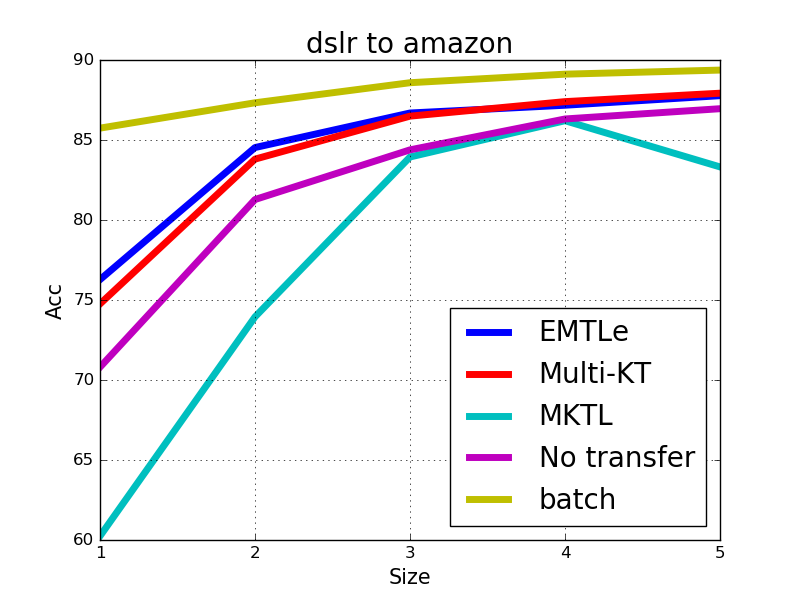
\includegraphics[width=0.30\textwidth]{pakdd/fig/dslrtoamazon.png}\label{b}
}
\subfloat[W$\rightarrow$A]{
	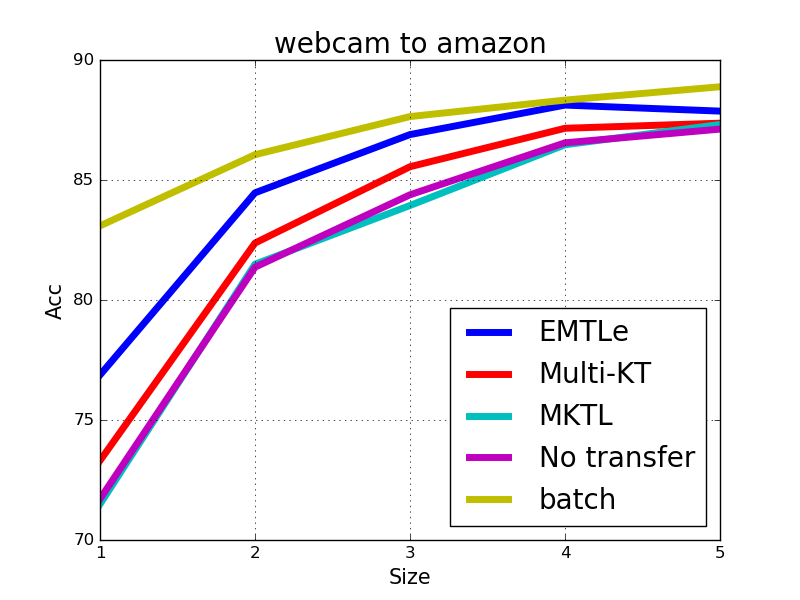
\includegraphics[width=0.30\textwidth]{pakdd/fig/webcamtoamazon.png}\label{c}
}\\
\subfloat[A$\rightarrow$C]{
	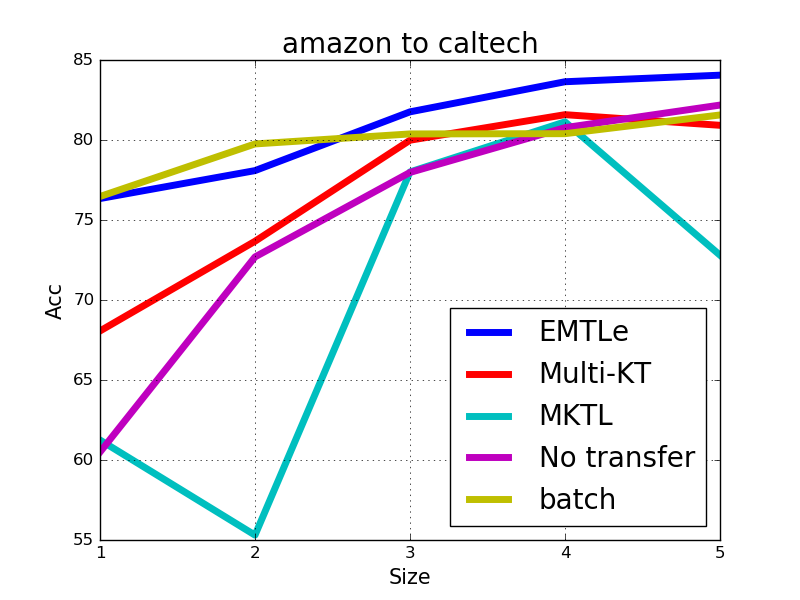
\includegraphics[width=0.30\textwidth]{pakdd/fig/amazontocaltech.png}\label{d}
}
\subfloat[D$\rightarrow$C]{
	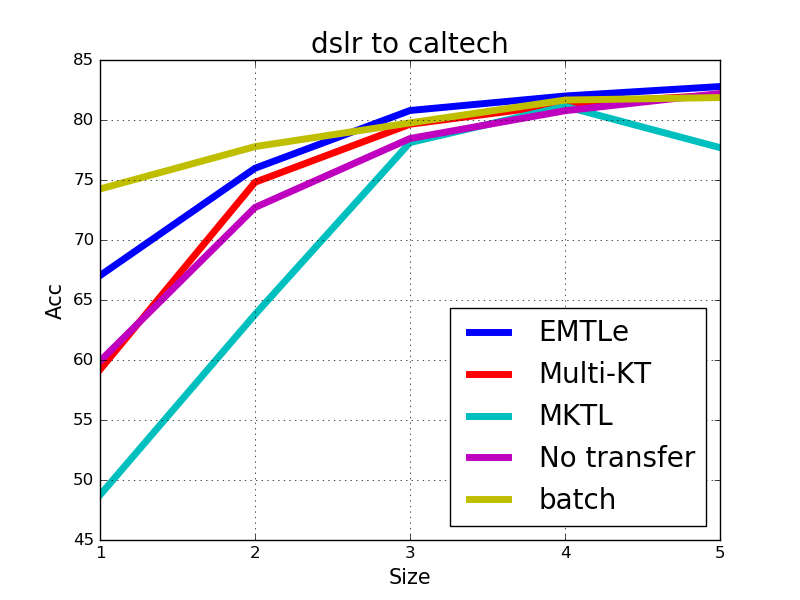
\includegraphics[width=0.30\textwidth]{pakdd/fig/dslrtocaltech.png}\label{e}
}
\subfloat[W$\rightarrow$C]{
	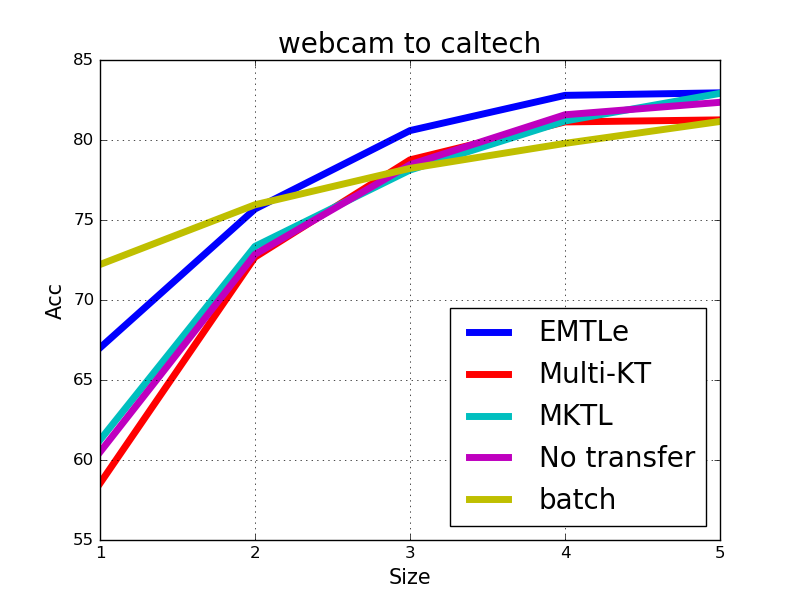
\includegraphics[width=0.30\textwidth]{pakdd/fig/webcamtocaltech.png}\label{f}
}\\
\subfloat[A$\rightarrow$D]{
	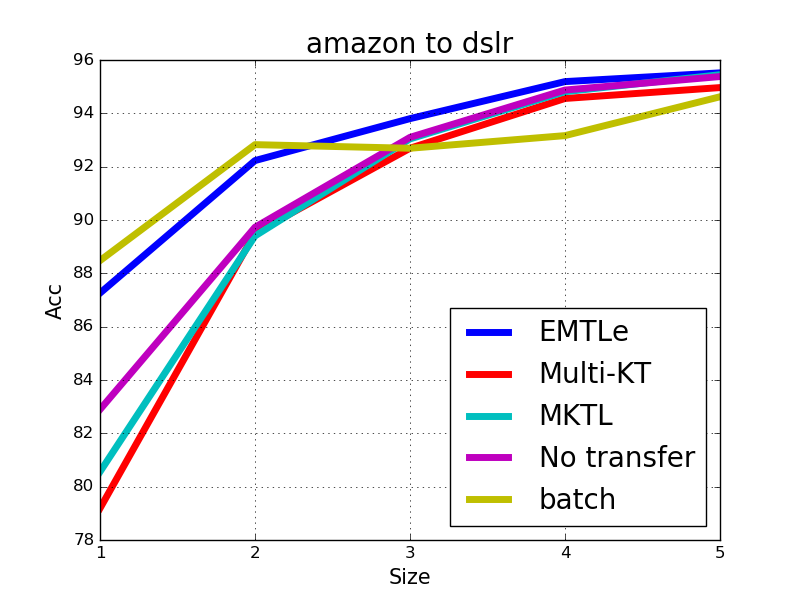
\includegraphics[width=0.30\textwidth]{pakdd/fig/amazontodslr.png}\label{g}
}
\subfloat[C$\rightarrow$D]{
	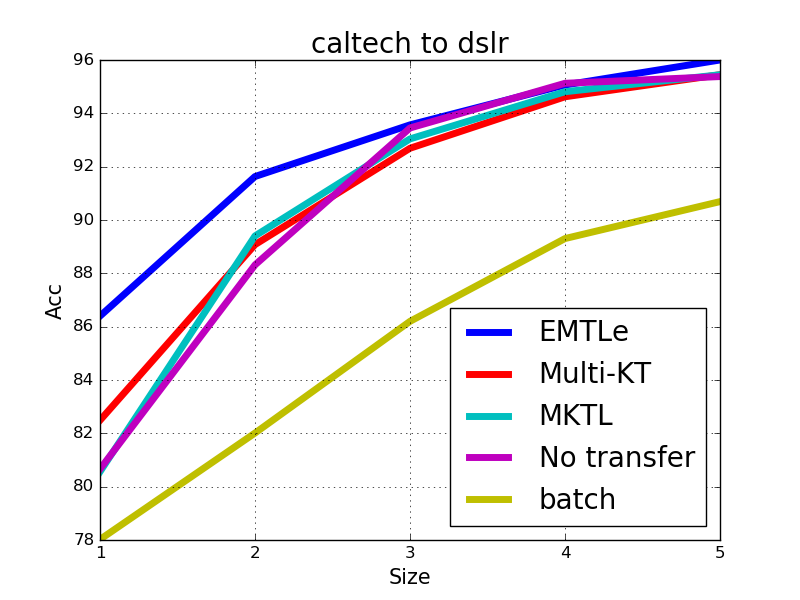
\includegraphics[width=0.30\textwidth]{pakdd/fig/caltechtodslr.png}\label{h}
}
\subfloat[W$\rightarrow$D]{
	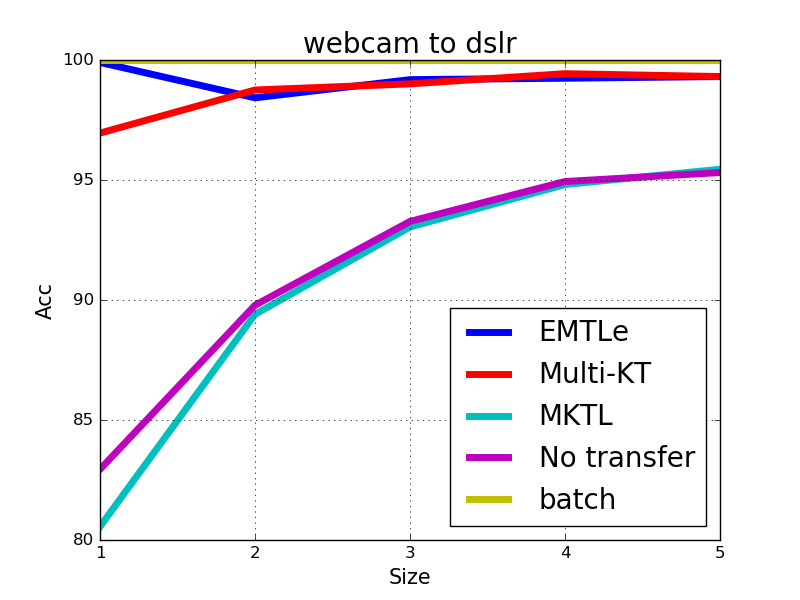
\includegraphics[width=0.30\textwidth]{pakdd/fig/webcamtodslr.png}\label{i}
}\\
\subfloat[A$\rightarrow$W]{
	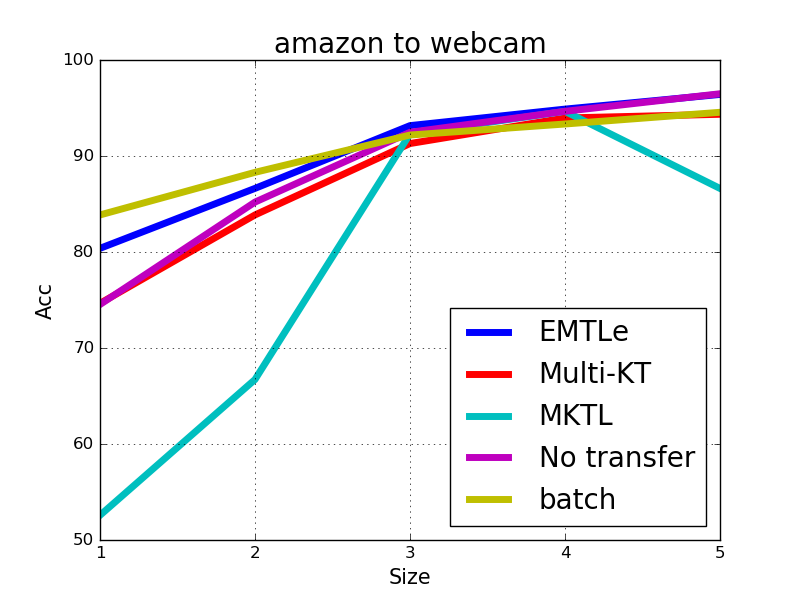
\includegraphics[width=0.30\textwidth]{pakdd/fig/amazontowebcam.png}\label{j}
}
\subfloat[C$\rightarrow$W]{
	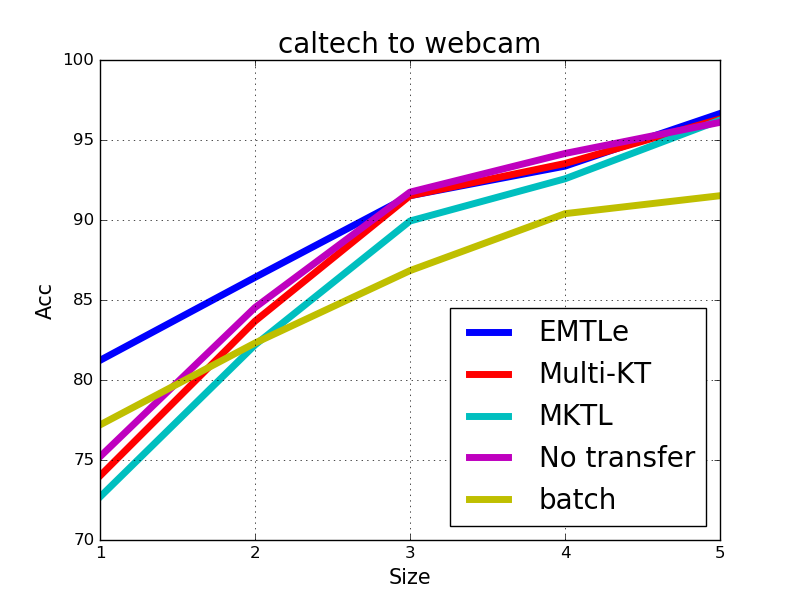
\includegraphics[width=0.30\textwidth]{pakdd/fig/caltechtowebcam.png}\label{k}
}
\subfloat[D$\rightarrow$W]{
	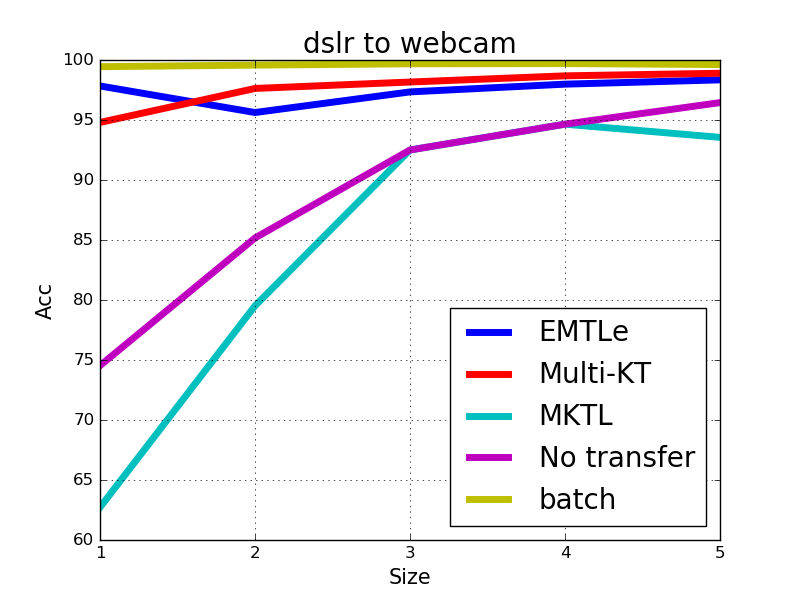
\includegraphics[width=0.30\textwidth]{pakdd/fig/dslrtowebcam.png}\label{l}
}
\caption{Recognition accuracy for HTL domain adaptation from a single source. 5 different sizes of target training sets are used in each group of experiments. A, D, W and C denote the 4 subsets in Table \ref{tab:class_info} respectively.}
\label{fig:exp}
\end{figure}

\textbf{Observation \& discussion:} EMTLe can significantly outperform other baselines especially with a small training set. %Moreover, in some groups of experiments, they even suffer from negative transfer on the small training set. 
As we have discussed above, when the training set is small, with the transfer parameter estimated by our $\ell_2$ penalty in our high-level objective functions, EMTLe has a strong generalization ability and performs better on the test data. As the training size increases, the variance of training data decreases and the affect of the $\ell_2$ penalty term become less significant. Therefore, EMTLe and the other two HTL baselines show similar performance. 
It is interesting to see that MKTL even falls into negative transfer even with 5 training examples per class in some experiments. We found that, MKTL is more sensitive to the variance of the training data. Its performance is not as stable as Multi-KT and EMTLe over the 10 experiments. Because MKTL needs to learn more hyperparameters than Multi-KT and EMTLe, even though the training size increases, it may not be able to obtain a good model. 
In some experiments, we can see that EMTLe can even outperform the Batch method which can access more information and is expected to outperform the other methods under the setting of HTL.

\subsection{Transfer from Multiple Source Domains}
As we mentioned, EMTLe can exploit knowledge from different types of source classifiers which could greatly extend our choice of the source domain under the HTL setting. In this subsection, we show that EMTLe can successfully transfer the knowledge from two different types of source classifiers. Meanwhile, MKTL and ``No Transfer" are used as our baseline. 

In this experiment, we assume that there is no single source domain that can cover all 13 classes in our target domain and we have to select source models from different source domains. Specifically, the 13 classes are selected from two different domains separately (6 from DSLR and 7 from Webcam) according to Table \ref{tab:class_gen}. Similar to our previous experiment configurations, we only use Caltech and Amazon as the target domains. We show the experiment results in Figure \ref{fig:exp2}.
% Table generated by Excel2LaTeX from sheet 'Sheet1'
\begin{table}[htbp]
	\centering
	\caption{The selected classes of the two source domains and the classifier type of the source model.}
	\begin{tabular}{|c|c|c|}
		\hline
		& class & classifier\\
		\hline
		DSRL& monitor,bike, helmet,calcu,headphone,projector & Logistic\\\hline
		Webcam&keyboard,mouse,phone,backpack,mug,bottle,laptop&SVMs\\ \hline
		
	\end{tabular}%
	\label{tab:class_gen}%
\end{table}%
\begin{figure}[h]
	\centering
	\subfloat[D+W $\rightarrow$ A]{
		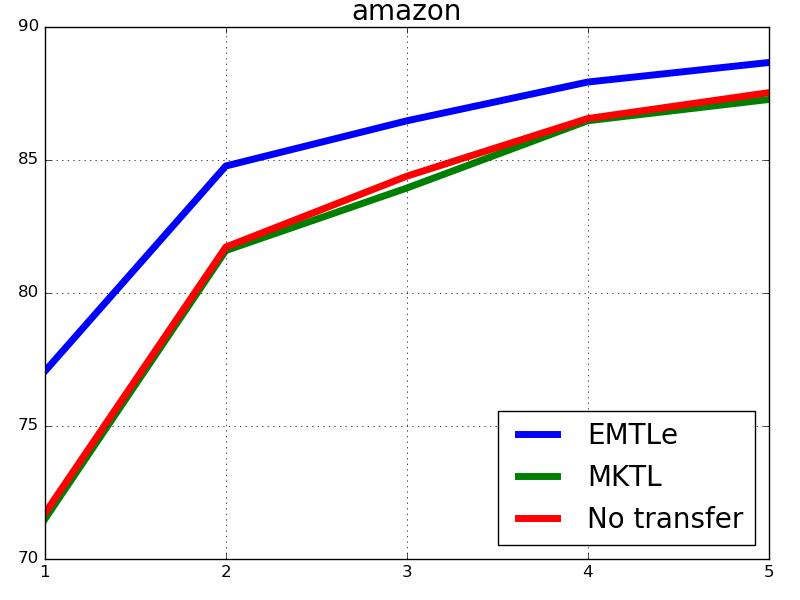
\includegraphics[width=0.5\textwidth]{pakdd/fig/multi_amazon.png}\label{a2}
	}
	\subfloat[D+W $\rightarrow$ C]{
		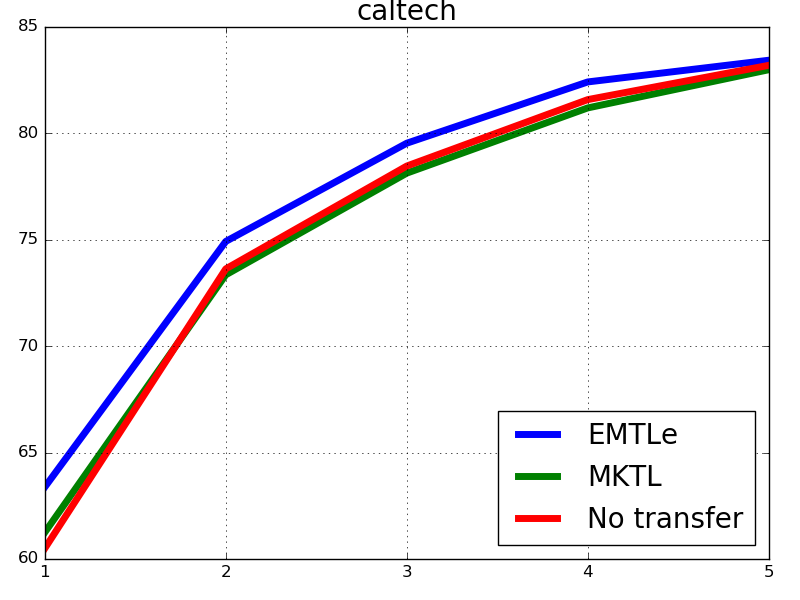
\includegraphics[width=0.5\textwidth]{pakdd/fig/multi_caltech.png}\label{b2}
	}\\
	\caption{Recognition Accuracy for Multi-Model \& Multi-Source experiment on two target datasets. }
	\label{fig:exp2}
\end{figure}

\textbf{Observation \& discussion:} In our multi-source scenario, it is more difficult to leverage the knowledge from the source models as the models are trained from different domains separately. From the results we can see that, EMTLe can still exploit the knowledge from the source models despite the types of the source classifiers while MKTL can hardly leverage the source knowledge. EMTLe uses a simple way to leverage the source models and BO can help us better estimate the transfer parameter. However, MKTL uses a sophisticated feature augmentation and has more hyperparameters to estimate. Without sufficient training data, it is difficult for MKTL to measure the importance of each source model and exploit the knowledge from the models.






\section{Summary}
In this chapter, we propose a method, EMTLe that can effectively transfer the knowledge under the HTL setting. We focus on the effectiveness and compatibility issues for HTL problems. We propose our auxiliary bias strategy to let our model exploit the knowledge from different types of source classifiers. The transfer parameter of EMTLe is estimated by bi-level optimization method using our novel high-level objective function which allows our model to better exploit the knowledge from source models. Experiment results demonstrate that EMTLe can effectively transfer the knowledge even though the size of training data is extremely small.

